%provide an overview of the data collection process (figures are preferred) 
In this section, we discuss how we collected the data set used in this study.
\begin{figure*}[h]
    \centering
    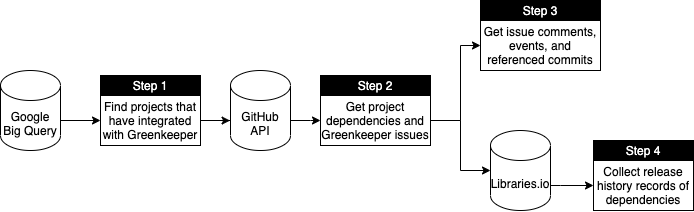
\includegraphics[width=12cm]{images/data_collection.png}
    \caption{Data collection overview}
    \label{fig:data_collection}
\end{figure*}
\par
~\subsection{Greenkeeper Issue Reports}\label{sec.data.issue_reports}
We use Google Big Query\footnote{https://cloud.google.com/bigquery} to find 12,134 GitHub projects that have integrated with Greenkeeper. From this list of repositories, we use the GitHub API\footnote{https://docs.github.com/en/free-pro-team@latest/rest} to retrieve the repository information, including the projects development and run-time dependency version specifications, as well as all of the issue reports for the project authored by the Greenkeeper bot. This leaves us with 123,197 in-range breaking build issue reports. For each of these issue reports, we collect any comments that have been made on the issue report, as well as any events that occurred on the issue report. Issue events\footnote{https://docs.github.com/en/free-pro-team@latest/rest/reference/issues\#events} can be any actions that concerns the event, such as closing an issue or referencing the event on a pull request. In total, we collect 365,625 comments and 209,750 issue events. If there were any commits that referenced the issue report, we collect information on those commits, for a total of 17,623 commits.
~\subsection{Provider Package Releases}\label{sec.data.provider_releases}
After each of the projects development and run-time dependencies had been extracted, we collected each of the dependencies release history from \textit{libraries.io}\footnote{https://libraries.io/}. In total, we collect information on 556,742 releases across 7,361 unique dependencies.
\par
An overview of the data collection process is shown in Fig.~\ref{fig:data_collection} and the data set is summarized in Table \ref{tab:all_data}.
\begin{table}[h]
    \begin{center}
    \begin{tabular}{ c|c } 
        \textbf{Entity} & \textbf{Records} \\
        \hline
        Projects & 12,134 \\
        \hline
        In-range breaking build issue reports & 123,197 \\
        \hline
        Issue comments & 365,625 \\ 
        \hline
        Issue events & 209,750 \\ 
        \hline
        Referenced commits& 17,623 \\ 
        \hline
        Release Versions & 556,742 \\ 
        \hline
    \end{tabular}
    \end{center}
    \caption{
        \label{tab:all_data} Summary of data
    }
\end{table}

